\documentclass{beamer}

\usetheme{Warsaw}
%\usetheme{CambridgeUS}

% modification history
% created on 18 sep 2011
% modified on 25 mar

%\usepackage{amsfonts, amsmath, amssymb}

%\setbeamertemplate{theorems}[numbered]
%\setbeamertemplate{theorems}[ams style] 
\usepackage[skins,breakable]{tcolorbox}
%\usepackage[normalem]{ulem}

%\usefonttheme[onlymath]{serif}                     // change the style of math font 

%=============set slide number=================
\addtobeamertemplate{navigation symbols}{}{
    \usebeamerfont{footline}
    \usebeamercolor[fg]{footline}
    \hspace{1em}
    \insertframenumber/\inserttotalframenumber
}
\setbeamercolor{footline}{fg=black}
\setbeamerfont{footline}{series=\bfseries}


%=============set footline=====================
\setbeamertemplate{footline}
{
  \leavevmode%
  \hbox{%
  \begin{beamercolorbox}[wd=.55\paperwidth,ht=2.25ex,dp=1ex,center]{author in head/foot}%
    \usebeamerfont{author in head/foot}\insertshortauthor
  \end{beamercolorbox}%
  \begin{beamercolorbox}[wd=.45\paperwidth,ht=2.25ex,dp=1ex,center]{title in head/foot}%
    \usebeamerfont{title in head/foot}\insertshorttitle
  \end{beamercolorbox}}%
  \vskip0pt%
}

%creating a rectangle box def
\newtcbox{\mybox}[1][red]{arc=0pt,outer arc=0pt,colback=#1!10!white,colframe=#1!50!black, boxsep=0pt,left=1pt,right=1pt,top=2pt,bottom=2pt,boxrule=0pt,bottomrule=1pt,toprule=1pt}

\newtcbox{\xmybox}[1][red]{arc=7pt,colback=#1!10!white,colframe=#1!50!black,before upper={\rule[-3pt]{0pt}{10pt}},boxrule=1pt,boxsep=0pt,left=6pt,right=6pt,top=2pt,bottom=2pt}
%the ``on line'' option doesn't work. so omitting it

%===== spacing =====

\def\extraspacing{\vspace{2mm} \noindent}
\def\vgap{\vspace{2mm}}
\def\hgap{\textrm{\hspace{1mm}}}

%===== tabbing =====

\def\tab{\hspace{2mm}}
\def\tabpos{\hspace{4mm} \= \hspace{4mm} \= \hspace{4mm} \= \hspace{4mm} \=
\hspace{4mm} \= \hspace{4mm} \= \hspace{4mm} \= \hspace{4mm} \= \hspace{4mm}
\kill}
\newcommand{\mytab}[1]{\begin{tabbing}\tabpos #1\end{tabbing}}

%===== blocks =====

% \newtheorem{theorem}{Theorem}
% \newtheorem{lemma}{Lemma}
% \newtheorem{corollary}{Corollary}
% \newtheorem{proposition}{Proposition}
% \newtheorem{definition}{Definition}
% \newtheorem{problem}{Problem}

\newcommand{\cbox}[2]{\begin{tcolorbox}[arc=0mm, colframe=#1!50!black, colback=#1!10!white]#2\end{tcolorbox}}
\newcommand{\minipg}[2]{\begin{center}\begin{minipage}{#1}#2\end{minipage}\end{center}}
\newcommand{\myfrm}[1]{\begin{frame}\begin{small}#1\end{small}\end{frame}} 
\newcommand{\myitems}[1]{\begin{itemize}#1\end{itemize}}
\newcommand{\myenums}[1]{\begin{enumerate}#1\end{enumerate}}
\newcommand{\myfig}[1]{\begin{figure}\centering #1\end{figure}}
    
%===== math macros =====
\newcommand{\bm}[1]{\textrm{\boldmath${#1}$}}
%\newcommand{\smat}[2]{\left[\begin{tabular}{#1}#2\end{tabular}\right]}
%\newcommand{\bmat}[2]{\left|\begin{tabular}{#1}#2\end{tabular}\right|}
\newcommand{\bmat}[1]{\begin{bmatrix}#1\end{bmatrix}}
\newcommand{\vmat}[1]{\begin{vmatrix}#1\end{vmatrix}}
\newcommand{\myeqn}[1]{\begin{eqnarray}#1\end{eqnarray}}
\newcommand{\set}[1]{\{#1\}}

\def\eps{\epsilon}
\def\fr{\frac}
\def\lc{\lceil}
\def\lf{\lfloor}
\def\rc{\rceil}
\def\rf{\rfloor}
\def\Pr{\textrm{\boldmath$Pr$}}
\def\expt{\textrm{\boldmath$E$}}
\def\real{\mathbb{R}}
\def\int{\mathbb{Z}}
\def\*{\star}
\def\tO{\tilde{O}}

\DeclareMathOperator*{\argmin}{arg\,min}
\DeclareMathOperator*{\polylg}{polylg}
\DeclareMathOperator*{\polylog}{polylog}
\DeclareMathOperator*{\intr}{\cap}

\def\nn{\nonumber}
\def\mit{\mathit}


%===== misc =====

\def\done{\hspace*{\fill} $\framebox[2mm]{}$}	% end of proof
\def\ttt{\texttt}

%===== coloring =====
\newcommand{\red}[1]{\textcolor{red}{#1}}
\newcommand{\bred}[1]{\textcolor{red}{\bf #1}}
\newcommand{\blue}[1]{\textcolor{blue}{\bf #1}}

\usepackage{color}
\usepackage{graphicx}
\usepackage{multirow}
\usepackage{wrapfig}
\usepackage[skins,breakable]{tcolorbox}

\def\done{\hfill$\square$}
\def\ttt{\texttt}
\def\vgap{\vspace{5mm}}

\def\best{\mit{best}}
\def\size{\mit{size}}
\def\sort{\mit{sort}}

\title[DATABASE SYSTEM PRINCIPLES]{Query Processing 6:\\ Join Order Optimization}

\author[Yufei Tao @ NTU]{Yufei Tao}
\institute[]{\url{https://www.cse.cuhk.edu.hk/~taoyf}}
\date{}

% \def\dtm{\mathit{d\mbox{-}tm}}
% \def\ftm{\mathit{f\mbox{-}tm}}
\def\bestext{\mathit{best\mbox{-}ext}}

\begin{document}
%-------------------------------------------------------------
\begin{frame}
    \titlepage
%     \begin{tcolorbox}[arc=0mm, colframe=green!50!black, colback=green!10!white] 
%     \end{tcolorbox}
\end{frame}
%-------------------------------------------------------------
\begin{frame}
\begin{small}
    In this lecture, we will discuss the \blue{join order} problem, which is the most important query rewriting optimization in database systems.

    \vgap

    Recall:
    \cbox{blue}{
        \blue{Query rewriting} converts the original query to an equivalent query using laws of relational algebra.
    }
    %\vgap
\end{small}    
\end{frame}
%-------------------------------------------------------------
\myfrm{
    \xmybox{Laws of natural joins}

    \vgap

    Let $\red{R_1}, \red{R_2}$, and $\red{R_3}$ be relations.

    \vgap

    \blue{Commutativity:} $R_1 \bowtie R_2 = R_2 \bowtie R_1$ \\
    \blue{Associativity:} $R_1 \bowtie (R_2 \bowtie R_3) = (R_1 \bowtie R_2) \bowtie R_3$ \\

    \vgap

    Therefore: $(R_1 \bowtie R_2) \bowtie R_3 = (R_1 \bowtie R_3) \bowtie R_2 = (R_2 \bowtie R_3) \bowtie R_1$.

    \vgap

    \cbox{blue}{
        In general, we can compute the natural join of several relations by ordering the relations arbitrarily.
    }
}
%-------------------------------------------------------------
\myfrm{
    \cbox{blue}{
        Various join orderings can have extremely different I/O costs.
    }

    \cbox{green}{
        \blue{Example:}\\
        Relations $\red{R_1(A,B)}$, $\red{R_2(C,D)}$, $\red{R_3(A,D)}$, each having 1000 tuples, where $A$ is the primary key of $R_1$.

        \vgap

        \blue{Join order 1:} $R_1 \bowtie R_2 \bowtie R_3$ \\
        The intermediate relation $\red{R_4} = R_1 \bowtie R_2$ has $1000^2 = 10^6$ tuples!

        \vgap

        \blue{Join order 2:} $R_1 \bowtie R_3 \bowtie R_2$ \\
        The intermediate relation $\red{R_5} = R_1 \bowtie R_3$ has at most $1000$ tuples.

        %\vgap

        \cbox{blue}{
        Join order 1 is expected to be significantly more expensive.}
    }
}
%-------------------------------------------------------------
\myfrm{
    %In general, let $\red{R_1}, \red{R_2}, ..., \red{R_k}$ be $\red{k}$ relations.

    \cbox{blue}{
        Let $\red{S}$ be a set of relations. An \blue{ordering} of $S$ is a permutation of the relations in $S$.
    }
    %Number of orderings $= k!$.

%    \vgap

    \cbox{blue}{
        Fix an arbitrary ordering $\red{\pi} = (R_1, R_2, ..., R_t)$ where $t \ge 2$.
        \myitems{
            \item For each $\red{i} \in [2, t]$, $\red{R_1 \bowtie R_2 \bowtie ... \bowtie R_i}$ is a \blue{prefix} of $\pi$. The \blue{join size} \bred{of the prefix} is $|R_1 \bowtie R_2 \bowtie ... \bowtie R_i|$, i.e., the number of tuples output by the join defined by the prefix.

            \item The \blue{penalty} \bred{of $\pi$} is the sum of the join sizes of its $t-1$ prefixes.
        }
    }

    \cbox{blue}{
        \blue{The Join Order Problem:} Given $\red{k}$ relations $\red{R_1}, \red{R_2}, ..., \red{R_k}$, find an ordering of $\set{R_1, .., R_k}$ with the smallest penalty.
    }
}
%-------------------------------------------------------------
% \myfrm{
%     \cbox{green}{
%         \blue{Example:}
%         Relations $\red{R_1(A,B)}$, $\red{R_2(C,D)}$, $\red{R_3(A,D)}$. \\
%
%         %\vgap
%
%         \begin{tabular}{cc}
%             \begin{minipage}{0.45\linewidth}
%                 There are 6 join orders:
%                 \myenums{
%                     \item $R_1 \bowtie R_2 \bowtie R_3$ \\[-1mm]
%                     \item $R_1 \bowtie R_3 \bowtie R_2$ \\[-1mm]
%                     \item $R_2 \bowtie R_1 \bowtie R_3$ \\[-1mm]
%                     \item $R_2 \bowtie R_3 \bowtie R_1$ \\[-1mm]
%                     \item $R_3 \bowtie R_1 \bowtie R_2$ \\[-1mm]
%                     \item $R_3 \bowtie R_2 \bowtie R_1$
%                 }
%                 Each join order corresponding to an ordering of $\set{R_1, R_2, R_3}$.
%             \end{minipage}
%             &
%             \begin{minipage}{0.45\linewidth}
%                 The penalty of the ordering $(R_2, R_1, R_3)$ equals the sum of $|R_2 \bowtie R_1|$ and $|R_2 \bowtie R_1 \bowtie R_3|$.
%             \end{minipage}
%         \end{tabular}
%     }
% }
%-------------------------------------------------------------
\myfrm{
    \cbox{blue}{
        Each ordering corresponds to a ``left-deep'' query plan. The \bred{join size of a prefix} is the output size of a join operation in the plan. The  \bred{penalty of the ordering} is the total output size of all the joins in the query plan. The join order problem essentially aims to minimize the total output size of the \bred{intermediate} joins (i.e., ``non-root'' joins in the plan). (\blue{Think}: why?).
    }
    \cbox{green}{
        \blue{Example}

        \vspace{-5mm}
        \begin{center}
            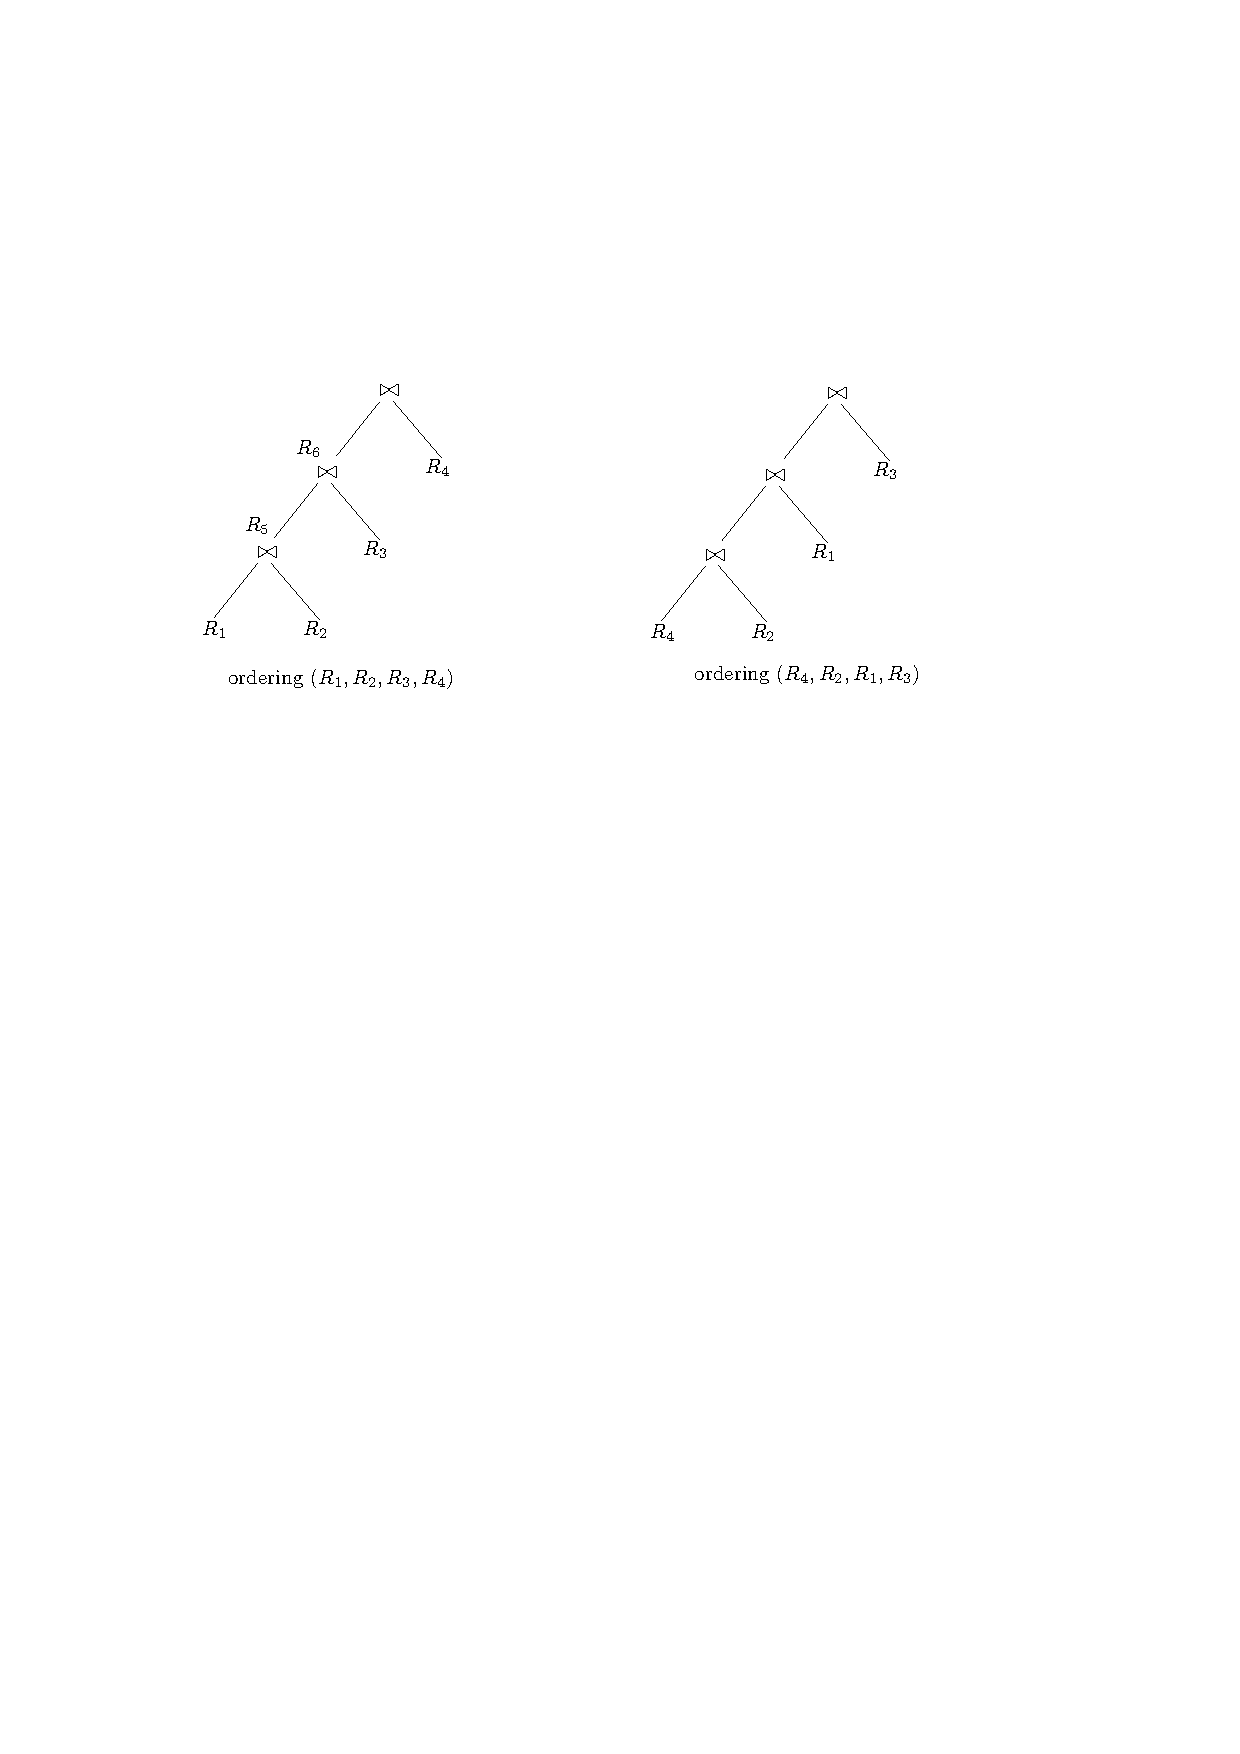
\includegraphics[height=30mm]{./artwork/ld1}
        \end{center}
        \vspace{-2mm}

        Consider the ordering $(R_1, R_2, R_3, R_4)$. The join size of the prefix $R_1 \bowtie R_2$ is $|R_5|$ (see $R_5$ in the figure), and that of the prefix $R_1 \bowtie R_2 \bowtie R_3$ is $|R_6|$. Note that $R_5$ and $R_6$ are the outputs of the intermediate joins in the query plan on the left.
    }
}
%-------------------------------------------------------------
\myfrm{
    Next, we will discuss how to solve the join order problem by assuming a \blue{size oracle}, which returns the output size of any join.

    \vgap

    \cbox{red}{
        Size oracles do not exist in reality. In reality, given any join, a database system can compute an \bred{estimate} of its output size. These estimates serve the purpose of size oracle. We will discuss such estimates in a tutorial.
    }

    \vgap

    Recall that the input to the problem has $\red{k}$ relations $\red{R_1}, \red{R_2}, ..., \red{R_k}$. The problem can be solved naively with $\red{k \cdot k!}$ calls to the size oracle (\blue{think}: how?).

    \vgap

    \cbox{blue}{
        We will show that the problem can be solved with less than $\red{k \cdot 2^k}$ oracle calls by dynamic programming.
    }
}
%-------------------------------------------------------------
\myfrm{
    Recall that $R_1, R_2, ..., R_k$ are the input to the join order problem.

    \vgap

    Let $\red{S}$ be a subset of $\set{R_1, R_2, ..., R_k}$ with size $|S| \ge 2$.

    \cbox{blue}{
        Define
        \myitems{
            \item $\red{\size(S)}$ as the size of the join involving all the relations in $S$;
            \item $\red{\best(S)}$ as the smallest penalty of all orderings of $S$.
        }
    }


}
%-------------------------------------------------------------
\myfrm{
    \cbox{green}{
        \blue{Example:} Consider $k = 4$, i.e., the input is $R_1, R_2, ..., R_4$. Assume that the size oracle returns the values in the left table.

        \vgap

        \begin{tabular}{cc}
            \begin{minipage}{0.47\linewidth}
                \begin{tabular}{c|c}
                    $S$ & join size \\
                    \hline
                    $R_1,R_2$ & 1000 \\
                    $R_1,R_3$ & 100 \\
                    $R_1,R_4$ & 50 \\
                    $R_2,R_3$ & 20 \\
                    $R_2,R_4$ & 100 \\
                    $R_3,R_4$ & 30 \\
                    $R_1, R_2, R_3$ & 1000 \\
                    $R_1, R_2, R_4$ & 1500 \\
                    $R_1, R_3, R_4$ & 800 \\
                    $R_2, R_3, R_4$ & 70 \\
                    $R_1, R_2, R_3, R_4$ & 20
                \end{tabular}
            \end{minipage}
            &
            \begin{minipage}{0.5\linewidth}
                For $S = \set{R_1, R_3, R_4}$, we have
                \myitems{
                    \item $\size(S) = 800$
                    \item $\best(S) = 830$, which is the penalty of the ordering $(R_3, R_4, R_1)$.
                }

                \vgap

                For $S = \set{R_1, R_2}$, we have $\size(S)$ $= \best(S) = 1000$.
            \end{minipage}
        \end{tabular}

    }
}
%-------------------------------------------------------------
\myfrm{ \label{slide:thm}
    \cbox{blue}{
        \blue{Theorem 1:} Let $\red{S}$ be a subset of $\set{R_1, ..., R_k}$ with $|S| \ge 2$. \\ If $|S| = 2$, then
        \myeqn{
            \best(S) = \size(S). \label{thm:1}
        }
        If $|S| > 2$, then
        \myeqn{
            \best(S) = \size(S) + \min_{\substack{\text{subset $\red{S'} \in S$}\\ \text{with $\red{|S'| = |S| - 1}$}}} \best(S'). \label{thm:2}
        }
    }

    \cbox{green}{
        \blue{Example:} Continuing on the example of the previous slide, we know that $\best(\set{R_1, R_3, R_4})$ equals $\size(\set{R_1, R_3, R_4}) = 800$ plus the minimum of
        \myitems{
            \item $\best(\set{R_1, R_3}) = \size(\set{R_1, R_3}) = 100$
            \item $\best(\set{R_1, R_4}) = \size(\set{R_1, R_4}) = 50$
            \item $\best(\set{R_3, R_4}) = \size(\set{R_1, R_4}) = 30$.
        }
    }
}
%-------------------------------------------------------------
\myfrm{
    \cbox{blue}{
        \blue{Corollary 2:} Let $\red{S}$ be a subset of $\set{R_1, ..., R_k}$ with $|S| \ge 3$. If $\best(S')$ is available for every subset $S' \subseteq S$ with $|S'| = |S| - 1$, we can compute $\best(S)$ with $|S| \le k$ oracle calls.
    }

    The corollary naturally implies the following algorithm for solving the join order problem.

    \vgap

    \blue{Step 1:} Find $\best(S)$ for every $S \subseteq \set{R_1, ..., R_k}$ with $\red{|S| = 2}$ \\ (one oracle call for each $S$).

    \vgap

    \blue{Step $\red{t \ge 2}$:} Find $\best(S)$ for every $S \subseteq \set{R_1, ..., R_k}$ with $\red{|S| = t+1}$ \\
    (at most $k$ oracle calls for each $S$).

    \vgap

    We obtain $\best(\set{R_1, ..., R_k})$ after Step $k - 1$.
}
%-------------------------------------------------------------
\myfrm{
    \cbox{green}{
        \blue{Example:} Consider $k = 4$, i.e., the input is $R_1, R_2, ..., R_4$. Assume that the size oracle returns the values in the left table. The right table illustrates the computation of the $\best$ values.

        \vgap

        \begin{tabular}{cc}
            \hspace{-5mm}
            \begin{minipage}{0.47\linewidth}
                \begin{tabular}{c|c}
                    $S$ & join size \\
                    \hline
                    $R_1,R_2$ & 1000 \\
                    $R_1,R_3$ & 100 \\
                    $R_1,R_4$ & 50 \\
                    $R_2,R_3$ & 20 \\
                    $R_2,R_4$ & 100 \\
                    $R_3,R_4$ & 30 \\
                    $R_1, R_2, R_3$ & 1000 \\
                    $R_1, R_2, R_4$ & 1500 \\
                    $R_1, R_3, R_4$ & 800 \\
                    $R_2, R_3, R_4$ & 70 \\
                    $R_1, R_2, R_3, R_4$ & 20
                \end{tabular}
            \end{minipage}
            &
            \hspace{-8mm}
            \begin{minipage}{0.47\linewidth}
                \begin{tabular}{c|c|c}
                    $S$ & $\best$ & \# oracle calls\\
                    \hline
                    $R_1,R_2$ & 1000 & 1\\
                    $R_1,R_3$ & 100 & 1 \\
                    $R_1,R_4$ & 50 & 1 \\
                    $R_2,R_3$ & 20 & 1\\
                    $R_2,R_4$ & 100 & 1\\
                    $R_3,R_4$ & 30 & 1\\
                    $R_1, R_2, R_3$ & 1020 & 2 \\
                    $R_1, R_2, R_4$ & 1550 & 2\\
                    $R_1, R_3, R_4$ & 830 & 2 \\
                    $R_2, R_3, R_4$ & 90 & 2\\
                    $R_1, R_2, R_3, R_4$ & 110 & 3
                \end{tabular}
            \end{minipage}
        \end{tabular}

        \vspace{2mm}
        \blue{Optimal join order:} $R_2 \bowtie R_3 \bowtie R_4 \bowtie R_1$.
    }
}
%-------------------------------------------------------------
\myfrm{
    \xmybox{Analysis}

    \vgap

    $\set{R_1, R_2, ..., R_k}$ has less than $\red{2^k}$ subsets of size at least 2. For every such subset $\red{S}$, the value $\best(S)$ is computed in one of the $k-1$ steps, and the computation requires at most $k$ oracle calls. The total number of oracle calls is therefore less than $k \cdot 2^k$.

    \vgap

    \cbox{red}{
        \blue{Remark:} Strictly speaking, the algorithm we have introduced only computes the capacity of the optimal ordering, rather than the optimal ordering itself. How do we (easily) fix this without increasing the number of oracle calls?
    }
}
%-------------------------------------------------------------
\end{document} 



